\chapter{MARCO CONCEPTUAL Y ESTADO DEL ARTE}

Este capítulo presenta el pensamiento computacional, que es el eje del Desafío Bebras, y cómo se organiza el Desafío a nivel internacional: su estructura, sus categorías y los criterios con que se diseñan sus tareas. Cierra con el estado del arte: el alcance del Desafío en el mundo y en América Latina, las plataformas que usan otros países y lo que se tomó de ellas, y qué distingue a un sistema de gestión de concursos.

\section{PENSAMIENTO COMPUTACIONAL}

\textcite[33]{wing2006} define el pensamiento computacional como los procesos de pensamiento con los que se formula un problema y se representa su solución de modo que un agente de procesamiento de información, humano o máquina, pueda ejecutarla. La definición lo separa de la programación: no se trata de enseñar a operar una computadora, sino de desarrollar una forma de razonar aplicable a cualquier área.

El pensamiento computacional comparte rasgos con el pensamiento matemático, en la forma de resolver problemas, y con el de ingeniería, en el diseño de sistemas que interactúan con el mundo real, pero se distingue de ambos por la naturaleza propia de la computación \parencite[35]{wing2006}. Por eso Bebras lo adoptó como eje: sus tareas no exigen saber programar, pero sí aplicar estrategias propias de la informática.

En el contexto escolar, \textcite[39]{grover2013} revisaron cómo evolucionó el concepto después de Wing. No hay una definición única, pero sí elementos que la literatura reconoce de forma amplia, entre ellos la abstracción y la generalización de patrones, la descomposición de problemas y las nociones algorítmicas. Este trabajo adopta cuatro de ellos como marco: la descomposición, el reconocimiento de patrones, la abstracción y el diseño de algoritmos. Una tarea Bebras puede poner en juego uno o varios.

\section{COMPONENTES DEL PENSAMIENTO COMPUTACIONAL}

Cada componente corresponde a una estrategia que el estudiante puede activar al resolver una tarea Bebras y a un aspecto que el autor de la tarea cuida al diseñarla.

\subsection{Descomposición}

Descomponer es dividir un problema complejo en partes más pequeñas que se pueden resolver por separado. \textcite[34]{wing2006} la considera una herramienta mental esencial, porque permite abordar problemas que nadie resolvería de una sola vez. En una tarea Bebras aparece cuando el estudiante identifica las partes de un problema que parece difícil y las resuelve una por una antes de unir la solución.

\subsection{Reconocimiento de patrones}

Reconocer patrones es identificar similitudes, regularidades o estructuras que se repiten dentro de un problema o entre problemas distintos. \textcite[39]{grover2013} lo incluyen, junto con la abstracción, entre los elementos del pensamiento computacional, porque permite trasladar una estrategia conocida a un problema nuevo. Al diseñar una tarea hay que calibrarlo: si el patrón es demasiado evidente, la tarea no evalúa nada; si está demasiado oculto, frustra al estudiante.

\subsection{Abstracción}

Abstraer es quedarse con la información relevante de un problema y descartar los detalles que no ayudan a resolverlo. \textcite[35]{wing2006} la considera el concepto más poderoso de la computación: pensar en varios niveles de abstracción es lo que distingue a quien piensa computacionalmente de quien solo programa. En Bebras aparece cuando el estudiante construye un modelo simplificado de una situación cotidiana para razonar sobre ella.

\subsection{Diseño de algoritmos}

Diseñar un algoritmo es definir una secuencia finita y ordenada de pasos que lleva a la solución. Para \textcite[33]{wing2006}, formular un problema de modo que admita una solución algorítmica ya es pensamiento computacional, la ejecute una persona o una máquina. En las tareas Bebras se evalúa cuando el estudiante debe ordenar una serie de acciones o construir una estrategia paso a paso.

La Figura~\ref{fig:componentes_pc} resume los cuatro componentes. Cada recuadro lleva una ilustración, el nombre del componente y, debajo, la idea que lo resume; se leen de izquierda a derecha y de arriba abajo, en el orden en que se describieron.

\newcommand{\componentepc}[3]{%
  \begin{minipage}[t]{0.45\textwidth}\centering
    \includegraphics[width=0.82\linewidth]{assets/ia/#1-r.png}\\[0.3em]
    {\color{huazul}\textbf{#2}}\\
    {\small\color{hugris}#3}
  \end{minipage}}

\begin{figure}[htbp]
    \centering
    \componentepc{pc-descomposicion}{Descomposición}{Dividir el problema en partes}\hfill
    \componentepc{pc-patrones}{Reconocimiento de patrones}{Encontrar lo que se repite}\\[1.4em]
    \componentepc{pc-abstraccion}{Abstracción}{Quedarse con lo esencial}\hfill
    \componentepc{pc-algoritmos}{Diseño de algoritmos}{Ordenar los pasos hacia la solución}
    \caption[Componentes del pensamiento computacional]{Componentes del pensamiento computacional considerados en el diseño de tareas del Desafío Bebras}
    \label{fig:componentes_pc}
\end{figure}

\section{EL DESAFÍO BEBRAS INTERNACIONAL}

\textcite{bebras} lo describe como el Desafío Internacional de Informática y Pensamiento Computacional, que se realiza cada año para acercar los conceptos fundamentales de la informática a estudiantes de primaria y secundaria de todo el mundo.

\subsection{Origen e historia de la organización}

El Desafío nació en Lituania en 2004, impulsado por la profesora Valentina Dagien\.e \parencite{dagienefutschek2008}. Su nombre, «Bebras», significa castor en lituano y alude al trabajo sistemático y la persistencia que busca fomentar. La Figura~\ref{fig:bebras2004} muestra una reunión de representantes de los primeros países, con sus banderas sobre la mesa, en los inicios de la organización.

\begin{figure}[htbp]
    \centering
    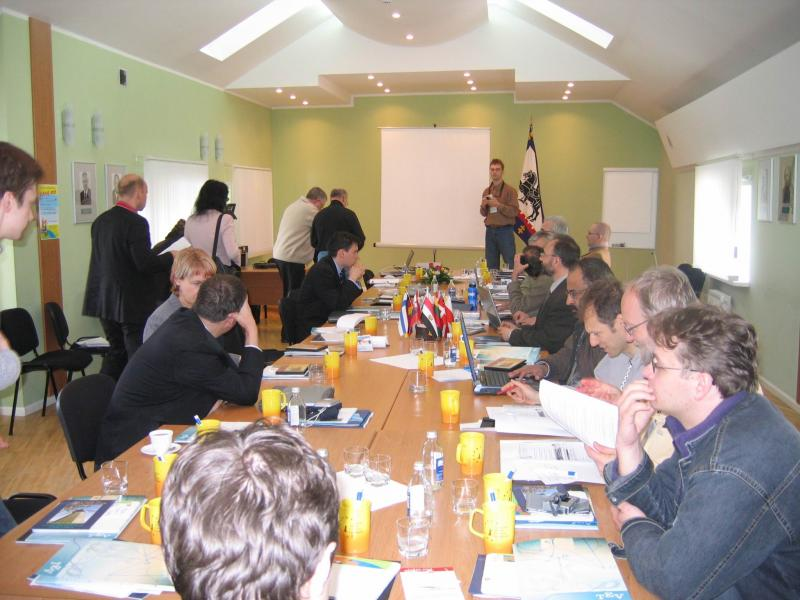
\includegraphics[width=0.65\textwidth]{assets/bebras2004.jpg}
    \caption[Primeros países de Bebras (2004)]{Primeros países vinculados al inicio de la organización Bebras en 2004. Galería oficial de Bebras \parencite{bebras}}
    \label{fig:bebras2004}
\end{figure}

En la edición 2023--2024 participaron 3\,936\,642 estudiantes de 70 países, y la comunidad contaba con 60 miembros plenos y 22 provisionales \parencite{bebrasstats2024}. En 2015 recibió el «Best Practices in Education Award» de Informatics Europe, patrocinado por Microsoft \parencite{bebras}.

\subsection{Modelo de gobernanza y el \emph{Bebras Task Workshop}}

Las tareas que cada país usa en su edición nacional no las crea un único equipo. Los representantes de los países miembro las proponen y revisan juntos en el \emph{Bebras Task Workshop}, un taller internacional anual \parencite{bebrastaskworkshops,dagienefutschek2008}. Así las tareas reflejan contextos culturales y niveles de dificultad diversos, y llegan al banco internacional ya revisadas. De ese banco, cada organizador nacional elige las que usará en su edición.

Por eso el sistema de Bebras Bolivia permite cargar y administrar tareas del banco internacional y adaptar sus enunciados al contexto boliviano cuando hace falta.

\section{ESTRUCTURA DEL DESAFÍO BEBRAS}

La estructura del Desafío está estandarizada a nivel internacional, aunque cada país puede adaptar algunos elementos, como el nombre de las categorías o el calendario.

\subsection{Categorías de participación}

\textcite{bebraseeuu} organiza el Desafío en seis categorías por edad, cada una con tareas ajustadas a su nivel: Kits (6--8), Castors (8--10), Benjamins (10--12), Cadets (12--14), Juniors (14--16) y Seniors (16--18). \textcite{bebrasperu} usa nombres propios de su cultura (Caral, Kuélap, Machu Picchu y Chan Chan) y conserva la progresión por edad. El modelo admite, por tanto, una adaptación local sin perder la comparabilidad internacional.

Bebras Bolivia siguió el mismo camino: sus seis categorías llevan nombres de la fauna del país, Guacamayo (5 a 8 años), Capibara (8 a 10), Titi (10 a 12), Jucumari (12 a 14), Yaguareté (14 a 16) y Kuntur (17 a 18), con los cursos que les corresponden en la Tabla~\ref{tab:categorias}. Como los rangos de edad se tocan en sus extremos, la categoría de cada estudiante se asigna por su curso, no por su edad exacta.

\subsection{Formato y duración}

El formato varía entre países y ediciones. En el estudio multinacional de \textcite[42]{izumirolo2017}, cada grupo de edad resolvía de 15 a 18 tareas (9 en el grupo de menor edad) en 45 a 55 minutos, con la misma cantidad de tareas, usualmente 5 o 6, en cada nivel de dificultad: fácil, medio y difícil; los estudiantes rendían en general supervisados por sus maestros. La mayoría de los países toma la prueba en línea, con corrección automática, pero algunos la toman en papel \parencite{bebrasstats2024}; por eso el objetivo de evaluación de este trabajo incluye formatos imprimibles para las aulas sin conexión.

\section{CRITERIOS PARA EL DISEÑO DE TAREAS BEBRAS}

Una tarea Bebras debe cumplir criterios pedagógicos que definen qué es un ejercicio válido. Esos criterios orientaron los campos, las validaciones y los tipos de respuesta que el banco de tareas del sistema ofrece al autor.

\subsection{Criterios pedagógicos fundamentales}

\textcite{dagienefutschek2008} discuten qué hace buena a una tarea Bebras: que esté vinculada de forma clara a conceptos de la informática, que se pueda resolver en pocos minutos y sin saber programar, y que resulte atractiva y adecuada para la edad a la que va dirigida. La Figura~\ref{fig:ciclo_bebras} resume ese ciclo de diseño: se parte de un concepto de informática, se lo convierte en una historia atractiva y en una tarea Bebras, se programa para hacerla interactiva, se resuelve y se discute por qué es informática; de esa discusión surge un concepto nuevo, con el que el ciclo vuelve a empezar. A estos criterios el sistema suma uno propio, necesario para corregir de forma automática: que la respuesta correcta se pueda verificar sin ambigüedad, por opción múltiple o por una interacción con un resultado único.

\begin{figure}[h]
    \centering
    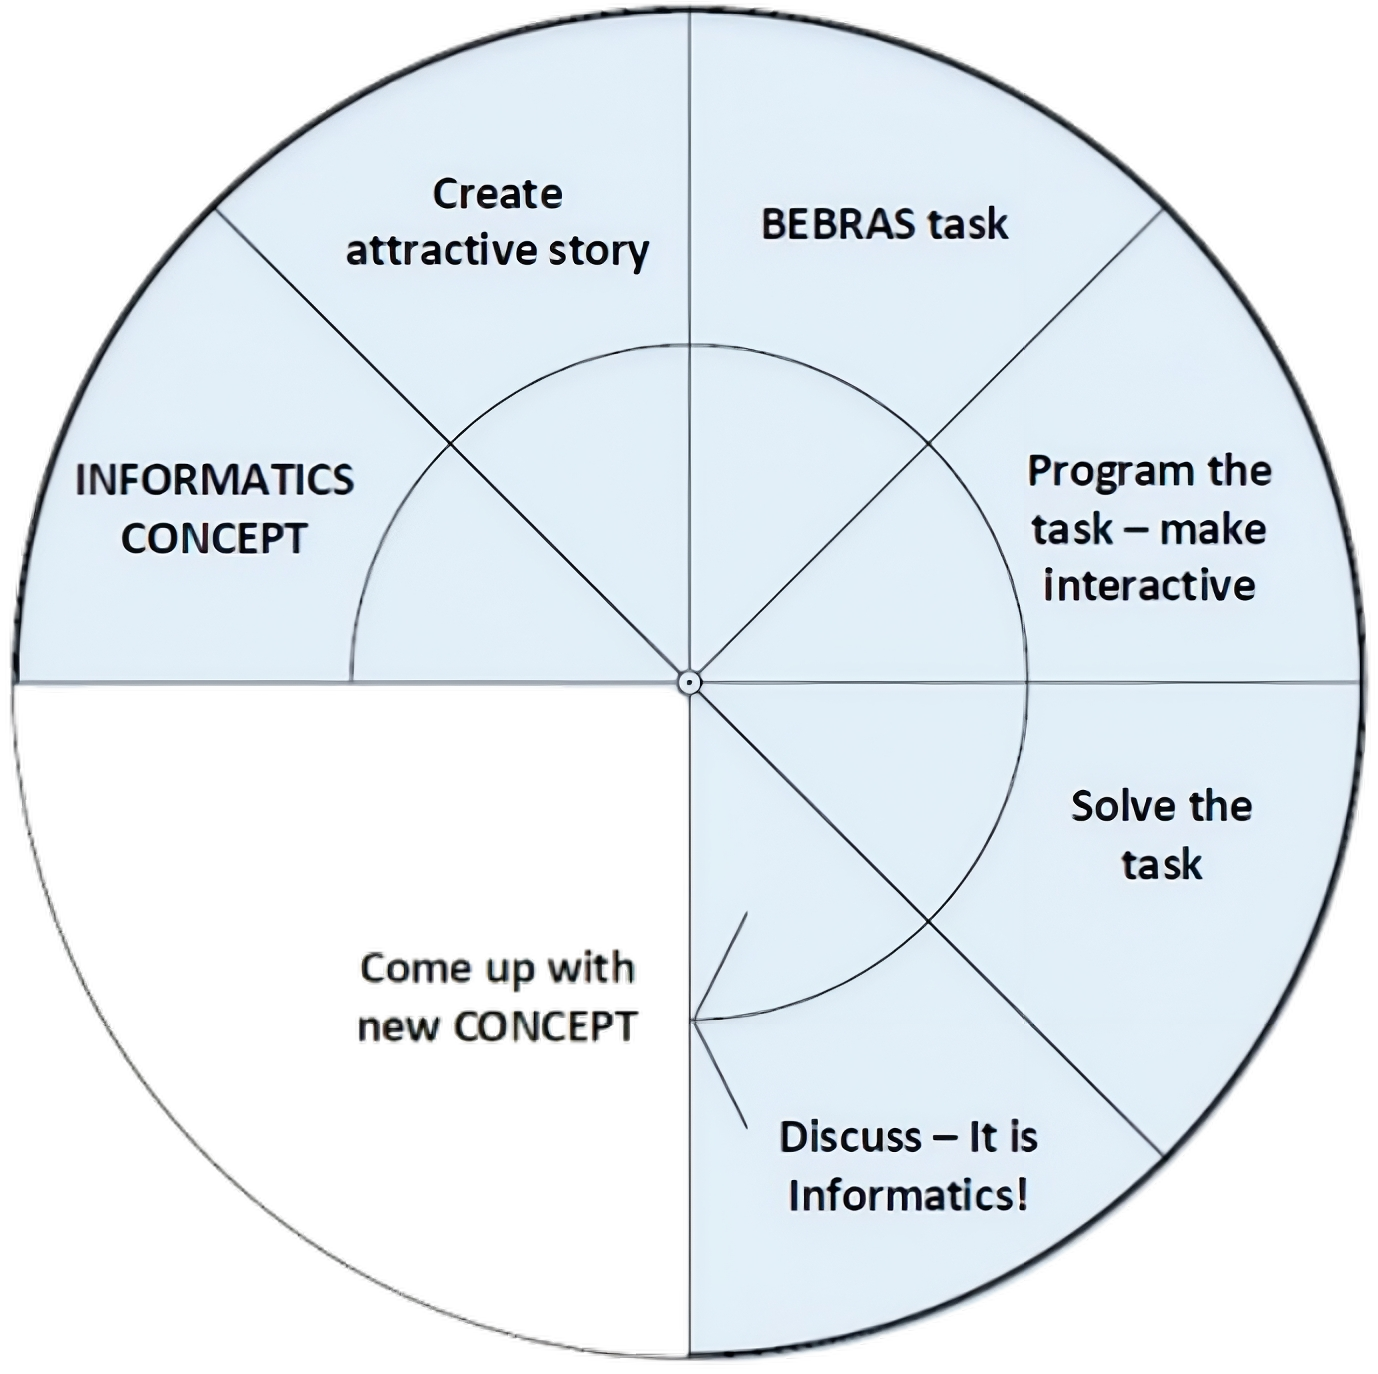
\includegraphics[width=0.5\textwidth]{assets/fig_dagiene2008.png}
    \caption[Ciclo de diseño de una tarea Bebras]{Ciclo de diseño de una tarea Bebras desde el concepto de informática hasta la comprensión del estudiante \parencite[p.~25]{dagienefutschek2008}}
    \label{fig:ciclo_bebras}
\end{figure}

\subsection{Tipos de tareas}

\textcite{dagienefutschek2008} distinguen dos tipos de tareas. Las de opción múltiple presentan un enunciado con un conjunto cerrado de alternativas, de las que solo una es correcta; son simples de implementar y de corregir. Las interactivas incorporan un elemento que el participante manipula en pantalla, como un grafo, una cuadrícula, una secuencia o un diagrama, para construir su respuesta; esa exploración favorece la comprensión de conceptos dinámicos como el ordenamiento, el recorrido de estructuras o la simulación de procesos. La Figura~\ref{fig:tipos_tareas} muestra ejemplos reales de ambos tipos. La tarea de opción múltiple (Figura~\ref{fig:tarea_opcion}) presenta una cadena de seis figuras y cuatro collares candidatos, rotulados de a) a d), entre los que se elige uno. En la tarea interactiva (Figura~\ref{fig:tarea_interactiva}) el participante actúa sobre esquemas de nodos unidos por varillas, en lugar de elegir entre alternativas escritas.

\begin{figure}[h]
    \centering
    \begin{subfigure}[b]{0.65\textwidth}
        \centering
        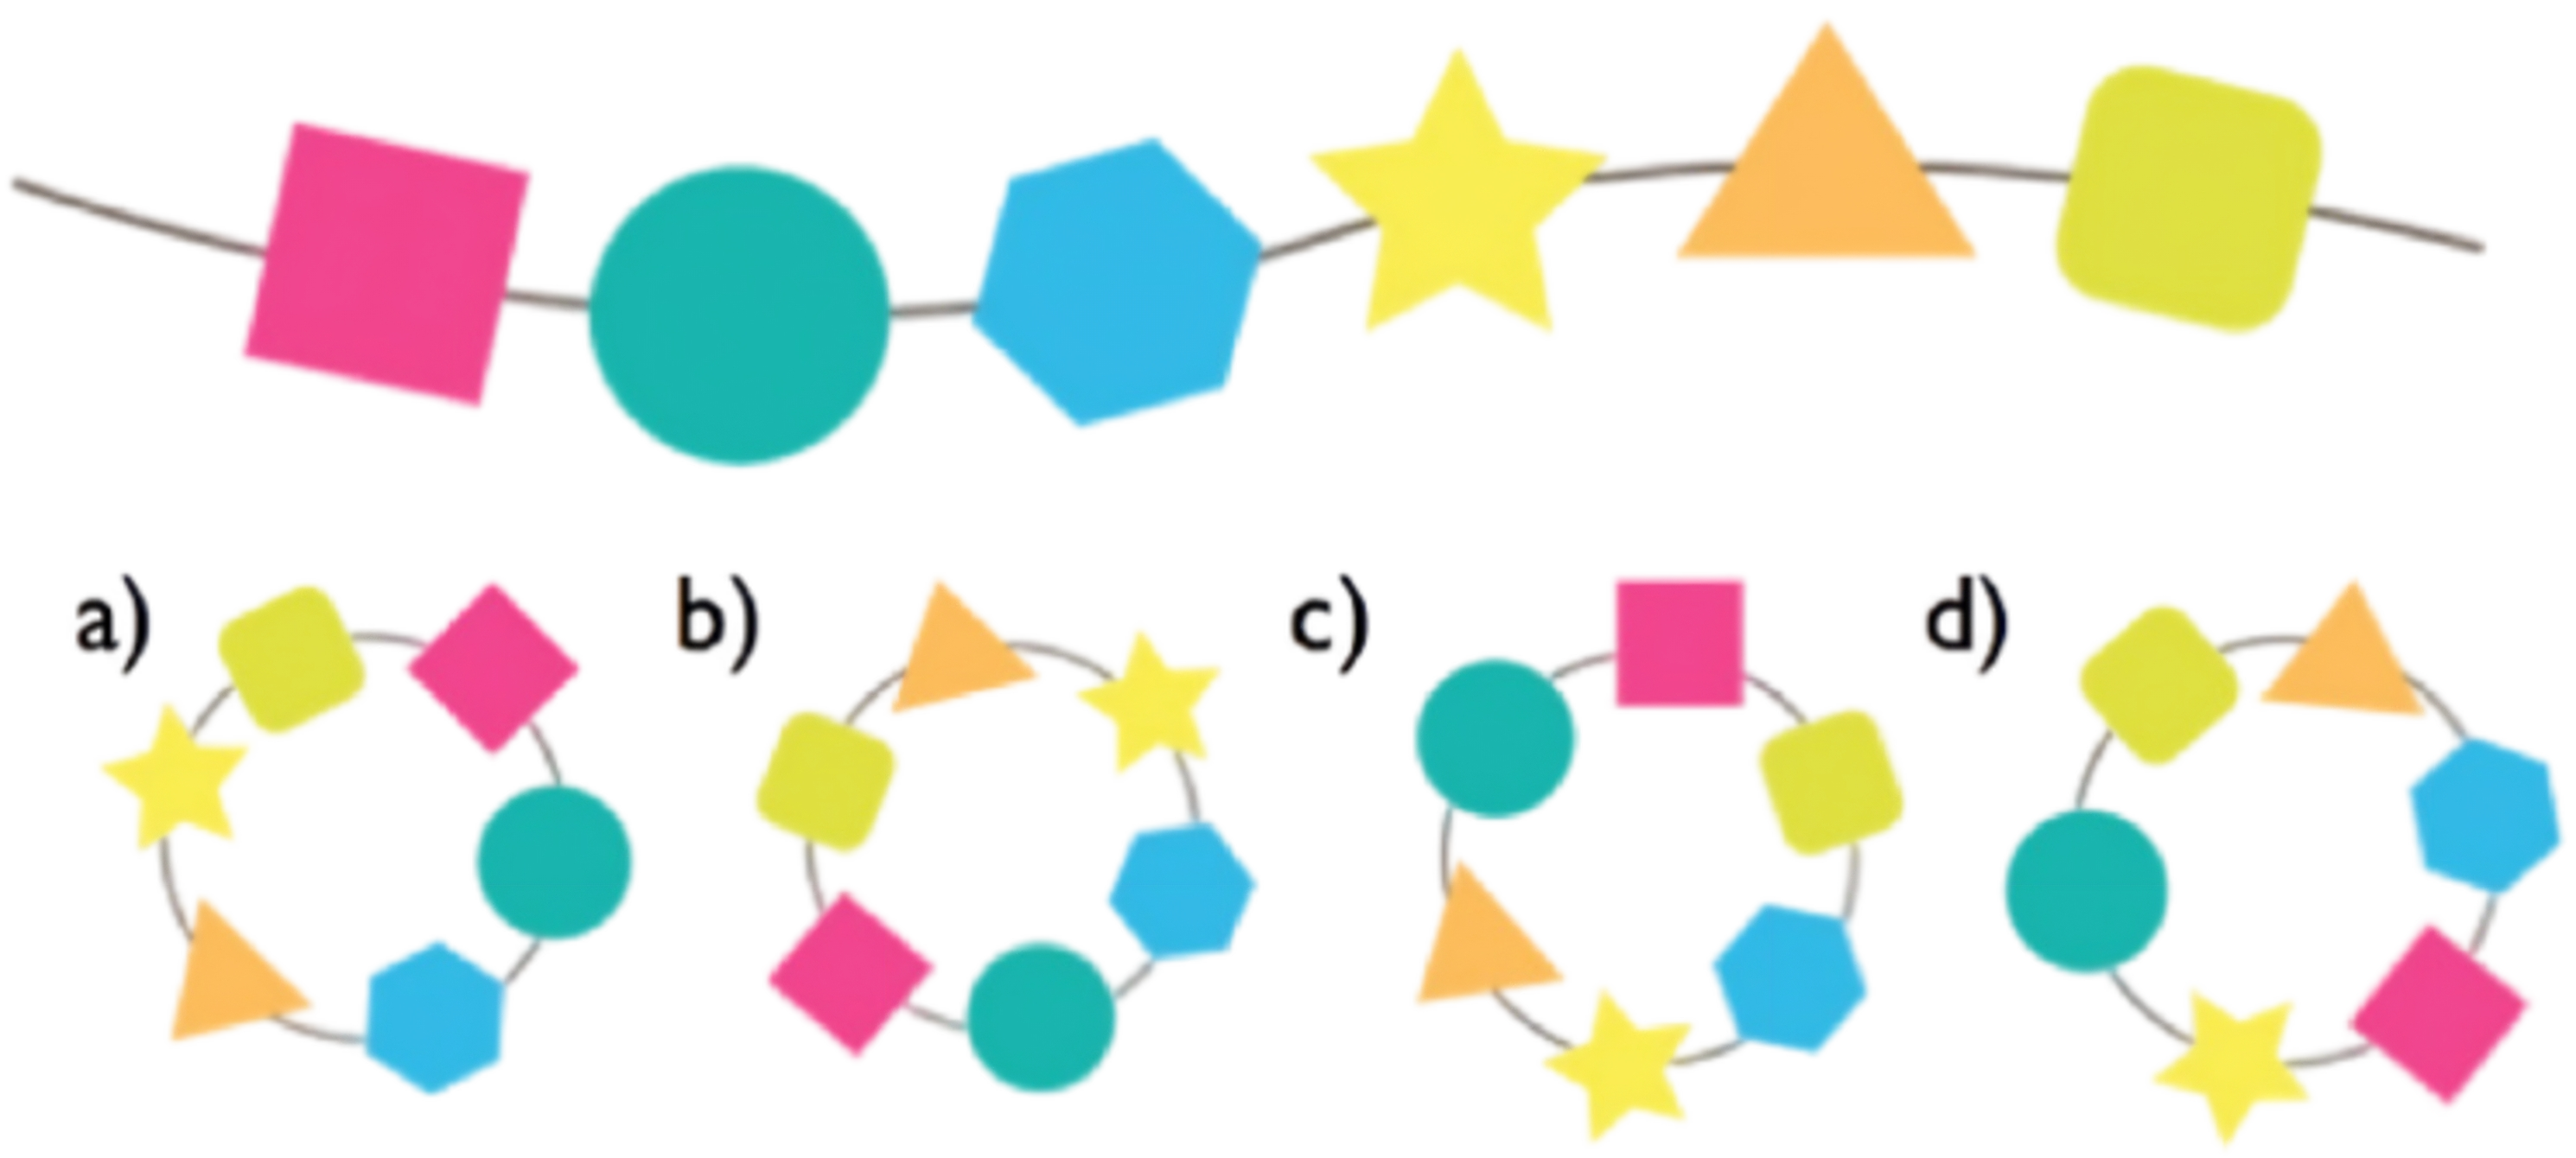
\includegraphics[width=\textwidth]{assets/fig_tarea_opcion.png}
        \caption{Tarea de opción múltiple (Task 2015-MY-01)}
        \label{fig:tarea_opcion}
    \end{subfigure}

    \vspace{0.5cm}

    \begin{subfigure}[b]{0.65\textwidth}
        \centering
        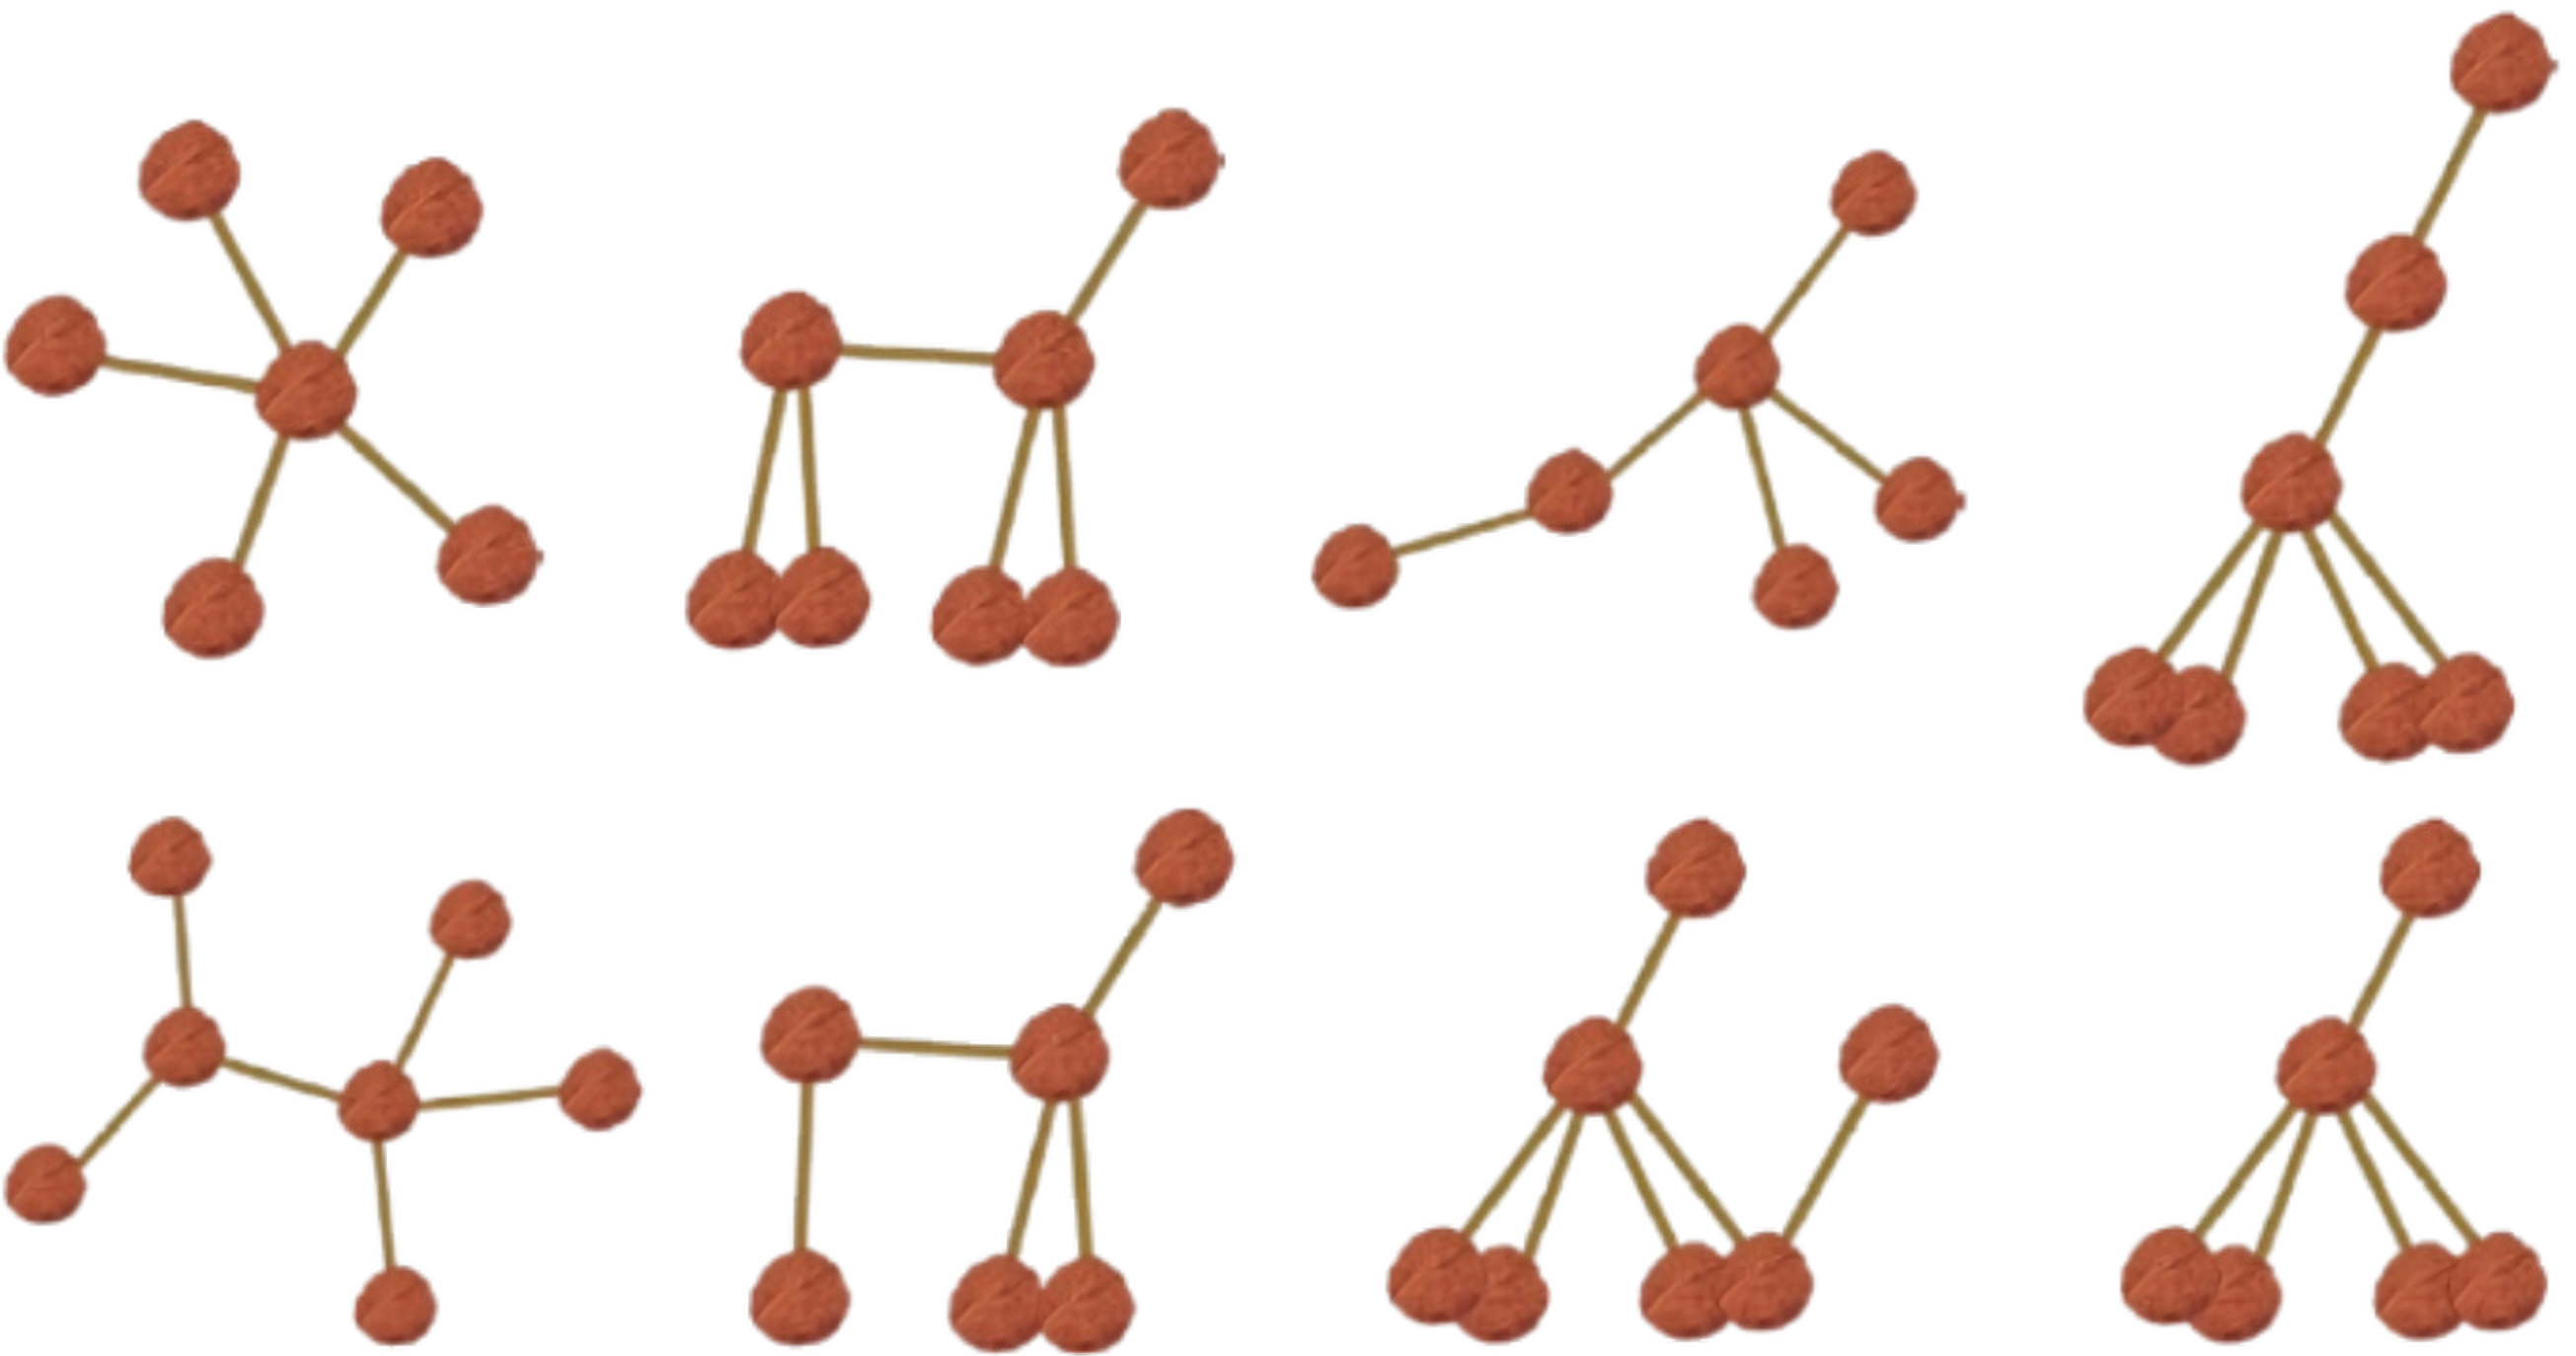
\includegraphics[width=\textwidth]{assets/fig_tarea_interactiva.png}
        \caption{Tarea interactiva (Task 2015-CZ-01)}
        \label{fig:tarea_interactiva}
    \end{subfigure}

    \caption[Ejemplos de tareas del Desafío Bebras]{Ejemplos de tareas del Desafío Bebras: opción múltiple e interactiva \parencite[pp.~46--47]{izumirolo2017}}
    \label{fig:tipos_tareas}
\end{figure}

\subsection{Niveles de dificultad y adecuación a la edad}

Asignar una tarea a un nivel de dificultad dentro de una categoría no es arbitrario: depende de la carga cognitiva que impone, es decir, de la cantidad de pasos hasta la solución, del grado de abstracción, de la información irrelevante del enunciado y de qué tan familiar es el contexto para esa edad \parencite{dagienestupuriene2016}. Esta calibración la hacen los autores de las tareas y el comité de revisión del taller internacional antes de que la tarea entre al banco oficial.

Como esa revisión ya ocurre en el taller internacional, el sistema de Bebras Bolivia no incluye un flujo propio de aprobación de tareas. El administrador carga tareas del banco ya validado, las adapta al contexto boliviano, les asigna una dificultad para cada categoría y las comprueba en el probador antes de usarlas en un desafío.

\section{ESTADO DEL ARTE}

El estado del arte revisa el alcance del Desafío Bebras en el mundo, su presencia todavía emergente en América Latina, las plataformas que usan los países miembro y los sistemas de gestión de concursos en línea.

\subsection{Alcance global del Desafío Bebras}

\textcite{izumirolo2017} hicieron el primer estudio multinacional de gran escala sobre el desempeño en tareas Bebras, con datos de 2014 y 2015 de 115\,400 estudiantes de 3.º a 12.º grado en siete países. Encontraron que las tareas de algoritmos y de representación de datos son entre el 75 y el 90~\% de las tareas, mientras que la abstracción, el paralelismo y la descomposición aparecen apenas en una o dos preguntas de algunos grupos de edad (Figura~\ref{fig:categorias_bebras}). Proponen esa clasificación como punto de partida para usar las tareas Bebras en el aula. En la Figura~\ref{fig:categorias_bebras}, cada grupo de barras es una categoría y cada color, un grupo de edad (mini, benjamin, cadet, junior y senior); la altura indica el porcentaje de tareas de esa categoría. Las dos primeras, algoritmos (ALG) y representación de datos (DR), superan ampliamente a las demás, y la abstracción (ABS) y el paralelismo (PAR) casi no aparecen.

\begin{figure}[h]
    \centering
    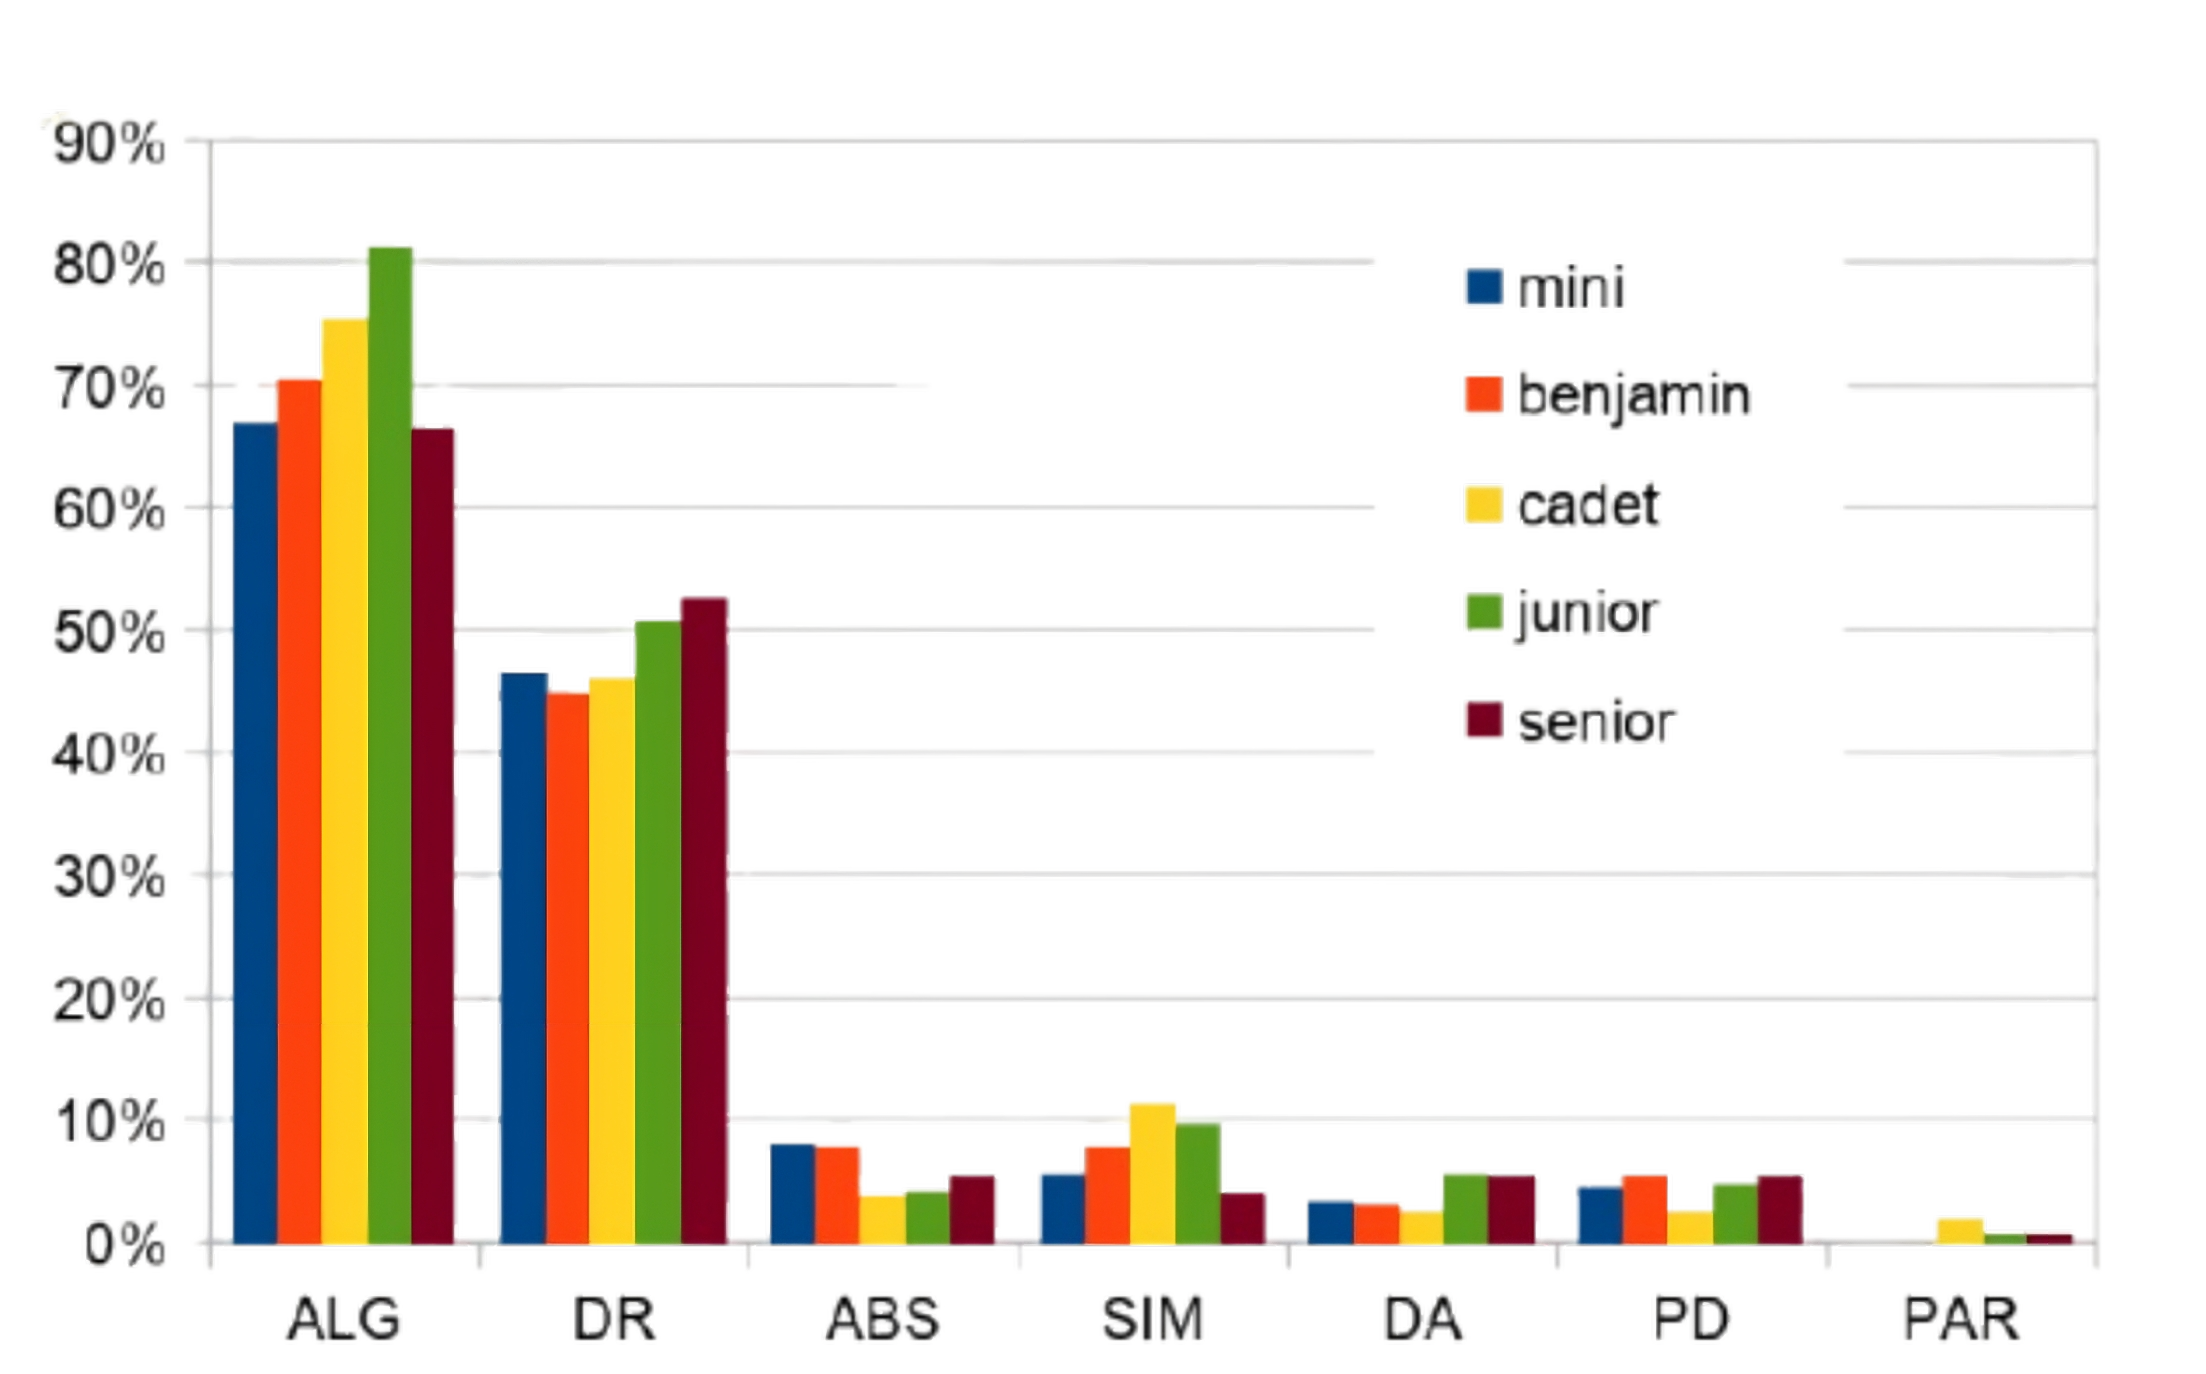
\includegraphics[width=0.6\textwidth]{assets/bebras_challenge_statistics.png}
    \caption[Distribución de categorías de pensamiento computacional en tareas Bebras]{Distribución de categorías de pensamiento computacional en tareas Bebras por grupo de edad \parencite[p.~48]{izumirolo2017}}
    \label{fig:categorias_bebras}
\end{figure}

\subsection{Bebras en América Latina}

La presencia de Bebras en América Latina es todavía menor que en Europa y Asia. Uruguay es uno de los países con mayor trayectoria: su programa nacional de pensamiento computacional usa las tareas Bebras, y \textcite{porto2024} analizaron sus resultados y la percepción de los docentes con perspectiva de género. Las tareas también se usan fuera de la competencia: \textcite{meza2024} validaron una prueba basada en tareas Bebras para medir el pensamiento computacional de estudiantes universitarios de primer año.

Bolivia se incorpora a la red en 2026; a la fecha de este documento no se ha realizado una edición nacional y la primera está prevista para el 13 de noviembre de 2026. Contar con un sistema propio para administrar el Desafío es una condición para que Bebras Bolivia se consolide como una iniciativa sostenible y comparable con las de otros países de la región.

\subsection{Estado de las plataformas tecnológicas Bebras}

No existe un sistema único que todos los países miembro deban usar. En la edición 2023--2024, 29 países usaron un sistema propio, 21 la plataforma Cuttle, 9 ViLLE, 7 Moodle, 4 el sistema francés y 4 tomaron la prueba en papel \parencite{bebrasstats2024}. Esta descentralización garantiza la autonomía de cada país, pero significa también que no hay una plataforma de referencia que se pueda adoptar tal cual.

\subsection{Análisis comparativo de plataformas Bebras de referencia}\label{sec:plataformas_referencia}

Por eso, para fundamentar las decisiones funcionales, de arquitectura y de interfaz, se analizaron cuatro implementaciones nacionales del Desafío Bebras al inicio del trabajo, antes de la primera iteración. Fue un análisis exploratorio, basado en sus sitios públicos y, cuando existía, en su código fuente, y buscó identificar sus módulos, su organización y su forma de interactuar con el usuario.

Los casos se eligieron porque su código o su información técnica es pública, porque llevan varias ediciones en uso y porque cubren las dos necesidades de Bolivia: administrar la competencia y comunicar. El objetivo no fue replicar una plataforma, sino reunir las buenas prácticas que cada una aporta.

\subsubsection{Plataforma de Francia --- Castor Informatique}

\emph{Castor Informatique}, mantenida por France-IOI, es una de las referencias más consolidadas de Bebras; su código, en PHP, es público bajo licencia MIT \parencite{bebrasfrancia,franceioirepo}. Separa con claridad los módulos de la competencia, de los maestros y de las preguntas, y prepara de antemano el material de la prueba para entregarlo con rapidez. De ella se tomó la idea de separar las áreas pública, administrativa y de evaluación, y la de servir el contenido ya preparado.

\subsubsection{Plataforma de Bélgica --- Rasbeb2}

\emph{Rasbeb2}, la plataforma de Bélgica, está escrita en Java y disponible bajo licencia MIT \parencite{bebrasbelgica,rasbeb2repo}; está organizada en módulos administrativos, de tareas interactivas y de documentación. Su principal aporte fue el diseño modular del flujo de la competencia, que separa inscripción, administración, rendición y evaluación. No se adoptó su tecnología, pero su organización guió la estructura funcional del sistema.

\subsubsection{Plataforma de Perú --- Bebras Perú}

La plataforma de Bebras Perú \parencite{bebrasperu} se centra en la comunicación institucional: presenta con claridad los niveles, los recursos, las orientaciones y la forma de inscribirse, pensando en maestros, unidades educativas y participantes. Su fortaleza es una organización de la información pensada para usuarios no técnicos, que sirvió de referencia para el sitio informativo.

\subsubsection{Plataforma de Estados Unidos --- Bebras Computing Challenge}

La plataforma de \textcite{bebraseeuu} combina la práctica libre con tareas de ediciones anteriores y un espacio de gestión para los responsables de cada institución. Su aporte fue el modelo de interacción con los ejercicios: cómo presenta el problema, cómo se navega entre tareas, cómo informa al usuario y cómo une la práctica con la evaluación. Sirvió de referencia para la experiencia del estudiante al resolver tareas.

\subsubsection{Síntesis de aportes}

Las plataformas revisadas responden a prioridades distintas: unas privilegian la administración completa de la competencia; otras, la difusión pública, la práctica libre o el contenido institucional. Ninguna resuelve por sí sola lo que necesita Bebras Bolivia, pero cada una aporta fortalezas concretas. Desarrollar un sistema propio no responde, entonces, a la falta de antecedentes, sino a la necesidad de reunir en una sola solución capacidades que hoy están repartidas entre distintas implementaciones nacionales. La Tabla~\ref{tab:retro_bebras} resume lo que se tomó de cada una.

\begin{table}[htbp]
\estilotabla
\begin{tabularx}{\linewidth}{>{\raggedright\arraybackslash}p{3.1cm} >{\raggedright\arraybackslash}p{4.6cm} >{\raggedright\arraybackslash}X}
\arrayrulecolor{huazul}\specialrule{1.4pt}{0pt}{0pt}
\rowcolor{hufondo}\textbf{Plataforma} & \textbf{Elemento rescatado} & \textbf{Aplicación} \\
\arrayrulecolor{hulinea}\midrule
Castor Informatique & Separación entre la competencia, los maestros y el banco de preguntas; entrega eficiente del contenido & Base para dividir el sistema en módulos y para entregar las tareas ya preparadas \\
Rasbeb2 & Organización modular del flujo de la competencia y soporte para tareas interactivas & Referencia para estructurar la inscripción, la rendición, la corrección y la administración en la plataforma del Desafío \\
Bebras Perú & Información clara para maestros, unidades educativas y participantes & Base para diseñar el sitio informativo según el tipo de usuario \\
Bebras Computing Challenge & Presentación de tareas, práctica previa y navegación entre ejercicios & Referencia para la experiencia del estudiante al resolver tareas y practicar \\
\arrayrulecolor{hulinea}\bottomrule
\end{tabularx}
\arrayrulecolor{black}
\caption[Elementos recuperados de plataformas Bebras de referencia]{Elementos recuperados de las plataformas Bebras de referencia y su aplicación en Bebras Bolivia}
\label{tab:retro_bebras}
\end{table}

\subsection{Sistemas de gestión de concursos en línea}

Un sistema de gestión de concursos en línea administra el ciclo completo de una competencia: el registro de participantes e instituciones, la preparación de las pruebas, su rendición en sesiones con tiempo limitado, la corrección automática y la publicación de resultados. Las cuatro plataformas analizadas comparten tres funciones: la identificación de los participantes, el banco de preguntas y la corrección de las respuestas.

Un sistema de gestión del aprendizaje (\textit{Learning Management System}, LMS) acompaña cursos en los que cada estudiante avanza a su ritmo. Una competencia como el Desafío, en cambio, reúne a muchos estudiantes en una misma ventana de tiempo, y de ahí salen tres requisitos de este sistema: atender muchas sesiones a la vez, controlar el tiempo de cada participante y no perder respuestas si se corta la conexión. El capítulo 4 muestra cómo los resuelve la arquitectura. La Figura~\ref{fig:cms_vs_lms} ilustra la diferencia: a la izquierda, un sistema de concursos, donde todos participan a la vez, con tiempo limitado y corrección inmediata; a la derecha, un sistema de aprendizaje, donde cada uno avanza a su ritmo durante meses y se sigue su progreso.

\begin{figure}[htbp]
    \centering
    \begin{minipage}[t]{0.48\textwidth}\centering
        {\color{huazul}\textbf{Sistema de gestión de concursos}}\\[0.4em]
        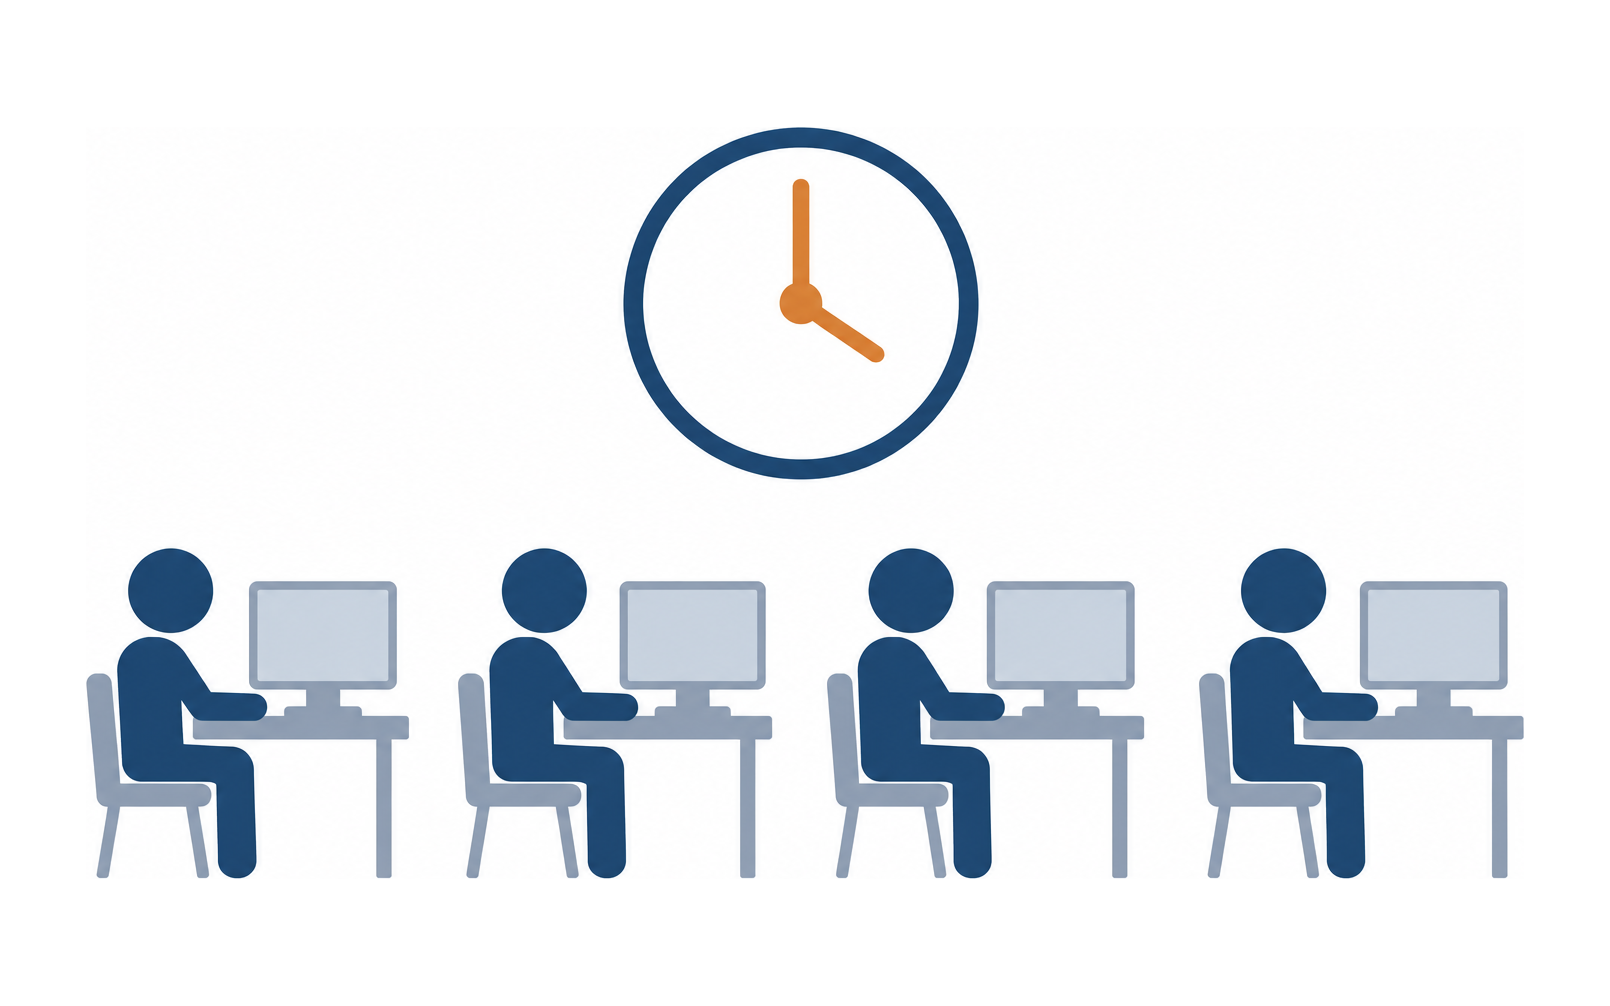
\includegraphics[width=\linewidth,height=3.6cm,keepaspectratio]{assets/ia/sistema-concursos-r.png}\\[0.2em]
        {\small\color{hugris}Todos a la vez · Tiempo limitado\\Corrección inmediata}
    \end{minipage}\hfill
    \begin{minipage}[t]{0.48\textwidth}\centering
        {\color{huazul}\textbf{Sistema de gestión del aprendizaje}}\\[0.4em]
        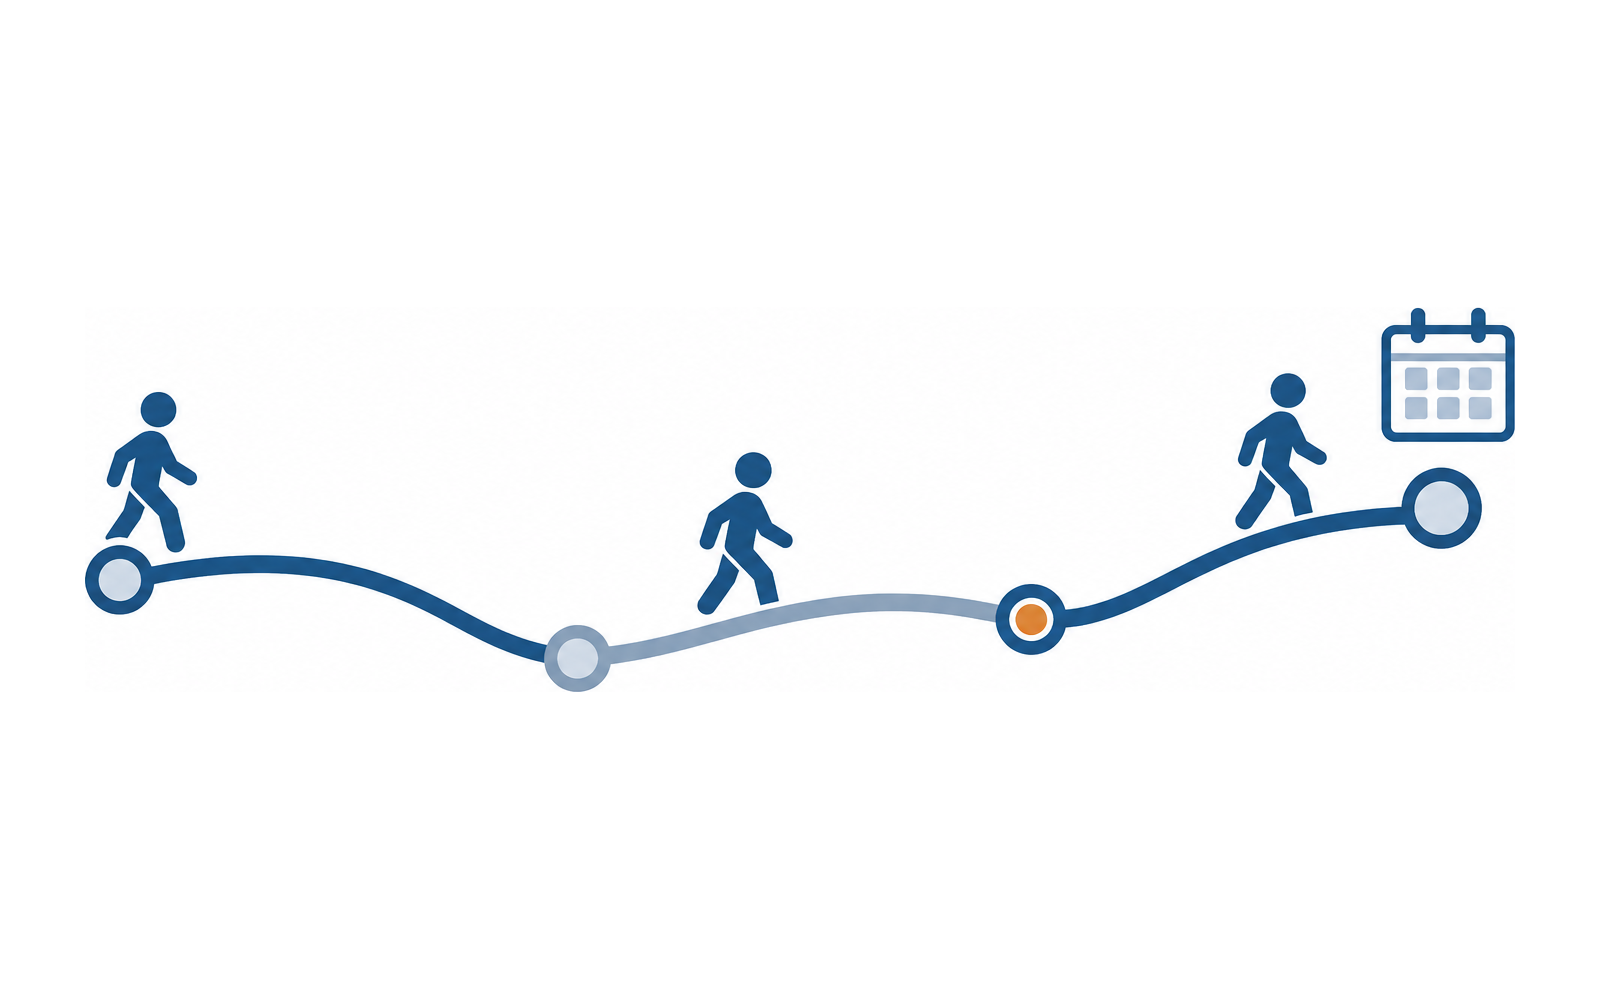
\includegraphics[width=\linewidth,height=3.6cm,keepaspectratio]{assets/ia/sistema-aprendizaje-r.png}\\[0.2em]
        {\small\color{hugris}Cada uno a su ritmo · Meses\\Seguimiento del progreso}
    \end{minipage}
    \caption[Sistema de gestión de concursos y sistema de gestión del aprendizaje]{Sistema de gestión de concursos frente a un sistema de gestión del aprendizaje}
    \label{fig:cms_vs_lms}
\end{figure}
